%!TEX root = *.tex
%%%%%%%%%%%%%%%%%%
% カウンタのリセット
\setcounter{figure}{0}
% 問題文
断面積$S$,長さ$L$の導体がある.
この導体には,電気量$-e$の自由電子が単位体積あたり\nn 個含まれるものとして,次の問いに答えよ.

\begin{enumerate}[(1)]
  \setlength{\leftskip}{-1.5zw}
  \setlength{\itemindent}{1zw}\setlength{\labelsep}{0.5zw}
  \setlength{\labelwidth}{1zw}\setlength{\leftmargin}{1zw}
  \setlength{\itemsep}{0.5\baselineskip}
  \item 図1のように,導体の両端に電圧$V$を加えた.
  \begin{enumerate}[(a)]
    \setlength{\leftskip}{-2.5zw}
    \setlength{\itemindent}{1zw}\setlength{\labelsep}{1zw}
    \setlength{\labelwidth}{1zw}
    \item 導体内に生じる電場の大きさはいくらか.その向きは図のA,Bのいずれか.
    \item 自由電子が電場から受ける力の大きさはいくらか.その向きはA,Bのいずれか.
  \end{enumerate}
  \item 自由電子は電場から力を受けるが,導体中の陽イオンからの抵抗力を受け,この2つの力がつりあって,自由電子は一定の速さで移動するとみなせる.
  この抵抗力の大きさが自由電子の速さに比例すると考え,その比例定数を$k$とする.
  \begin{enumerate}[(a)]
    \setlength{\leftskip}{-2.5zw}
    \setlength{\itemindent}{1zw}\setlength{\labelsep}{1zw}
    \setlength{\labelwidth}{1zw}
    \addtocounter{enumii}{2}
    \item 自由電子の速さはいくらか.
    \item 導体の断面を単位時間に通過する電子の数はいくらか.
    \item 導体を流れる電流の大きさはいくらか.
    \item オームの法則と(e)の結果を比較すると,導体の抵抗はいくらか.
  \end{enumerate}
  \item 導体の両端に加えた電圧により生じた電場は,抵抗力に逆らって自由電子を移動させる仕事をする.この仕事は,導体から発生するジュール熱と等しくなる.
  \begin{enumerate}[(a)]
    \setlength{\leftskip}{-2.5zw}
    \setlength{\itemindent}{1zw}\setlength{\labelsep}{1zw}
    \setlength{\labelwidth}{1zw}
    \addtocounter{enumii}{6}
    \item 電場が1個の自由電子に単位時間にする仕事はいくらか.
    \item 導体から単位時間に発生するジュール熱はいくらか.
  \end{enumerate}
\end{enumerate}

\begin{figure}[htbp]
  \centering
  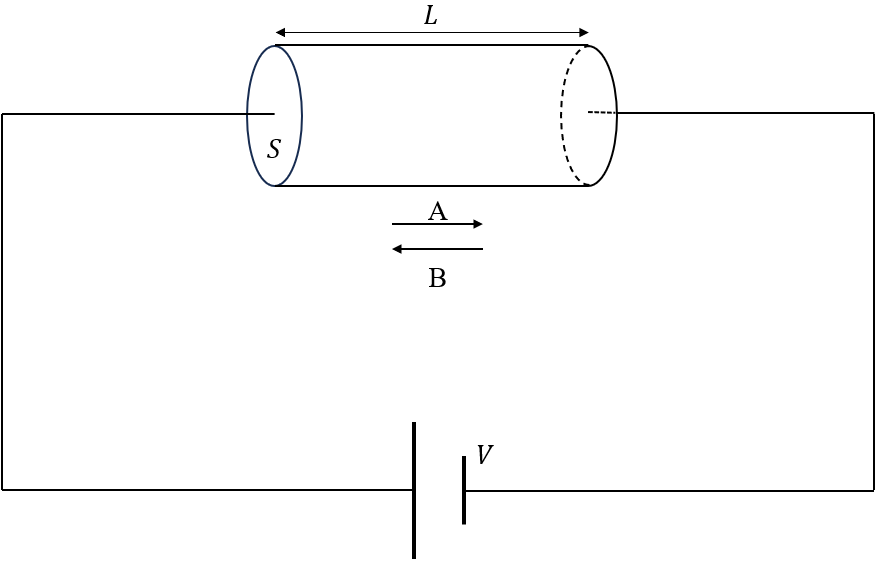
\includegraphics[width=0.8\textwidth]{../graphs/jumon_111.png}
  \caption{}
\end{figure}


% メモ
\begin{comment}

\end{comment}


%%%%%%%%%%%%%%%%%%
